\documentclass[11pt]{article}

\usepackage[margin=1.0in]{geometry}
\usepackage{enumitem}
\usepackage{tabularx}
\usepackage{pdfpages}
\usepackage{hyperref}
\hypersetup{
    colorlinks=true,
    linkcolor=blue,      
    urlcolor=cyan,
}

\urlstyle{same}

\newcommand{\code}[1]{\texttt{#1}}
\newcolumntype{L}[1]{>{\raggedright\arraybackslash}p{#1}}
\newcolumntype{C}[1]{>{\centering\arraybackslash}p{#1}}
\newcolumntype{R}[1]{>{\raggedleft\arraybackslash}p{#1}}

\begin{document}

\title{\textbf{Expression Calculator and Equation Solver} \\
    \url{https://github.com/stepheniskander/csc380project}}
\author{Nicholas Esposito \\ nesposi3@oswego.edu \and Stephen Iskander \\ siskande@oswego.edu}

\maketitle

\section{Project Description}
Our project is an expression calculator and equation solver.
The user can input mathematical expressions (e.g. \code{4*2+1}) to be evaluated to a numerical answer.
Expressions can also contain matrices or calculus operations such as integrals and derivatives.
If an expression contains one or more variables it will be simplified in terms of the variables (e.g. \code{(1*2)*x+(4-7) -> 2x-3}).
If the user inputs an equation containing a single variable, the program will solve for that variable.
The user can also input a system of equations that the program will solve if possible.

\par The program uses JavaFX for its user interface.
The main window is a simple command-prompt-like interface that the user types expressions or equations into.
Expressions are typed into a text field at the bottom of the window, and the expression as well as its evaluated answer are displayed in a text area above the input field.
The user can see their history in the output area so they can easily copy and paste previous expressions.
An additional window allows the user to graphically build matrices that will be inserted into the input field.
Systems of equations are handled on a separate tab to simplify inputting multiple equations.

\subsection{Stretch Goals}
The user can also use the program to graph functions.
Graphs are located on a separate tab.
The user inputs functions into an expandable list of functions and can choose what functions are visible on the graph.
A graph of all the visible functions is displayed next to the list of functions.
The window size and scale of the graph can be set manually or the program can attempt to set appropriate values.

\newpage

\section{System Requirements}

\begin{center}
\begin{tabular}{|L{.5in}|R{.5in}|L{5in}|}
\hline
\multicolumn{1}{|c|}{\textbf{Identifier}} & \multicolumn{1}{c|}{\textbf{Priority}} & \multicolumn{1}{c|}{\textbf{Description}} \\ \hline
REQ1  & 10 & Parsing user input into an expression. \\ \hline
REQ2  & 10 & Provide an interface for user to input expressions and see result.\\ \hline
REQ3  & 10 & Evaluate expression parse tree into numerical answer. \\ \hline
REQ4  & 9  & Evaluate an expression containing variables in terms of variables. \\ \hline
REQ5  & 8  & Solve an equation with a single variable. \\ \hline
REQ6  & 8  & Evaluate calculus operations numerically. \\ \hline
REQ7  & 7  & Evaluate calculus operations symbolically. \\ \hline 
REQ8  & 7  & Parse a matrix entered in text format ([[x y z] [a b c]]) \\ \hline
REQ9  & 7  & Perform matrix multiplication symbolically (i.e. each element is an expression). \\ \hline
REQ10 & 6  & Perform LU factorization on a matrix in order to solve a system of equations. \\ \hline
REQ11 & 5  & Provide a UI to simplify input of a system of equations. \\ \hline
REQ12 & 4  & Provide a graphical interface for building matrices. \\ \hline
REQ13 & 3  & Graph functions. \\ \hline
\end{tabular}
\end{center}

\newpage

\section{User Stories}

\begin{center}
\begin{tabular}{|L{.5in}|R{.5in}|L{5in}|}
\hline
\multicolumn{1}{|c|}{\textbf{Identifier}} & \multicolumn{1}{c|}{\textbf{Size}} & \multicolumn{1}{c|}{\textbf{Description}} \\ \hline
ST-1 & 3 pts & As a user, I can evaluate an expression by typing in the input field. \\ \hline
ST-2 & 6 pts & As a user, I can get a solution for an equation with a single variable. \\ \hline
ST-3 & 4 pts & As a user, I can evaluate an expression containing calculus operations numerically. \\ \hline
ST-4 & 4 pts & As a user, I can input a matrix in a text format. \\ \hline
ST-5 & 5 pts & As a user, I can perform matrix multiplication. \\ \hline
ST-6 & 6 pts & As a user, I can perform matrix multiplication in terms of variable matrix elements. \\ \hline
ST-7 & 4 pts & As a user, I can use a graphical interface to simplify creating a matrix. \\ \hline
ST-8 & 7 pts & As a user, I can solve a system of equations. \\ \hline
ST-9 & 4 pts & As a user, I can use a graphical UI to simplify entering a system of equations. \\ \hline
ST-10 & 9 pts & As a user, I can graph a function. \\ \hline
\end{tabular}    
\end{center}

\newpage

\section{Use Cases}

\begin{center}
\begin{tabular}{p{1.5in}p{5in}}
\hline
\textbf{Use Case UC-1}     & \textbf{EvaluateExpression} \\ \hline
Related Requirements: & REQ1, REQ2, REQ3 \\
Initiating Actor:     & User \\
Participating Actors: & GUI, ExpressionParser, Expression \\
Actor's Goal:          & To evaluate a mathematical expression typed into the calculator. \\
Preconditions:         & \begin{itemize}[nosep]
                         \item GUI is visible
                         \item ExpressionParser is initialized
                         \end{itemize} \\
Postconditions:        & \begin{itemize}[nosep]
                         \item Program is ready to evaluate another expression.
                         \end{itemize} \\ \hline
\end{tabular}

\begin{tabular}{p{.25in}p{.25in}p{5.8in}}
\multicolumn{3}{l}{Flow of Events for Main Success Scenario:} \\
$\rightarrow$ & 1. & The User types an expression into the input field and presses enter. \\
            & 2. & \code{include::ParseExpression} \\ 
$\leftarrow$  & 3. & Expression object evaluates to a number \\
$\leftarrow$  & 4. & GUI displays answer to User \\
\end{tabular}

\begin{tabular}{p{.25in}p{.25in}p{5.8in}}
\multicolumn{3}{l}{Flow of Events for Extensions:} \\
\multicolumn{2}{c}{\textbf{3a.}} & User entered an expression that cannot be evaluated \\
$\leftarrow$  & 1.           & Expression throws ArithmeticException
\end{tabular}
\end{center}


\newpage
\begin{center}
\begin{tabular}{p{1.5in}p{5in}}
\hline
\textbf{Use Case UC-2}     & \textbf{SolveEquation} \\ \hline
Related Requirements: & REQ4, REQ5, REQ3 \\
Initiating Actor:     & User \\
Participating Actors: & GUI, ExpressionParser, Expression, Equation \\
Actor's Goal:          & To solve an equation of a single variable. \\
Preconditions:         & \begin{itemize}[nosep]
                         \item GUI is visible
                         \item ExpressionParser is initialized
                         \end{itemize} \\
Postconditions:        & \begin{itemize}[nosep]
                         \item Program is ready to solve another equation.
                         \end{itemize} \\ \hline
\end{tabular}

\begin{tabular}{p{.25in}p{.25in}p{5.8in}}
\multicolumn{3}{l}{Flow of Events for Main Success Scenario:} \\
$\rightarrow$ & 1. & The User types an equation into the input field and presses enter. \\
              & 2. & \code{include::ParseExpression} \\ 
$\leftarrow$  & 3. & Each expression is simplified \\
$\leftarrow$  & 4. &Equation solve method is applied, and is evaluated to a number.  \\
$\leftarrow$  & 5. & GUI displays answer to User \\
\end{tabular}

\begin{tabular}{p{.25in}p{.25in}p{5.8in}}
\multicolumn{3}{l}{Flow of Events for Extensions:} \\
\multicolumn{2}{c}{\textbf{3a.}} & User entered an equation that cannot be solved \\
$\leftarrow$  & 1.           & Equation throws ArithmeticException \\

\multicolumn{2}{c}{\textbf{3b.}} & User entered an equation with more than one variable \\
$\leftarrow$  & 1.           & Equation solve method prints a warning string, aborts \\




\end{tabular}
\end{center}

\newpage

\begin{center}
\begin{tabular}{p{1.5in}p{5in}}
\hline
\textbf{Use Case UC-3}     & \textbf{ParseExpression} \\ \hline
Related Requirements: & REQ1 \\
Initiating Actor:     & GUI \\
Participating Actors: & ExpressionParser, Expression \\
Actor's Goal:          & To parse the incoming string into an evaluable expression. \\
Preconditions:         & \begin{itemize}[nosep]
		      \item  ExpressionParser is initialized
                         \end{itemize} \\
Postconditions:        & \begin{itemize}[nosep]
                         \item An Expression object is created and ready to be evaluated.
                         \end{itemize} \\ \hline
\end{tabular}

\begin{tabular}{p{.25in}p{.25in}p{5.8in}}
\multicolumn{3}{l}{Flow of Events for Main Success Scenario:} \\
$\rightarrow$ & 1. & String with Expression information comes from the GUI. \\
$\leftarrow$  & 2. & Diykstra's Shunting Yard Algorithm is used to convert the input in normal notation into Reverse Polish Notation\\
$\leftarrow$  & 3. & An Expression object is created that stores the  RPN in a Stack \\
\end{tabular}

\begin{tabular}{p{.25in}p{.25in}p{5.8in}}
\multicolumn{3}{l}{Flow of Events for Extensions:} \\
\multicolumn{2}{c}{\textbf{2a.}} & User entered an expression with invalid characters \\
$\leftarrow$  & 1.           & ExpressionParser throws NoSuchElementException\\

\multicolumn{2}{c}{\textbf{2b.}} & User entered an equation\\
 & 1.           & \code{extend::ParseEquation}\\

\end{tabular}
\end{center}

\newpage
\begin{center}
\begin{tabular}{p{1.5in}p{5in}}
\hline
\textbf{Use Case UC-4}     & \textbf{ParseEquation} \\ \hline
Related Requirements: & REQ5 \\
Initiating Actor:     & GUI \\
Participating Actors: & ExpressionParser, Expression,Equation \\
Actor's Goal:          & To parse the incoming string into an equation. \\
Preconditions:         & \begin{itemize}[nosep]
		      \item  ExpressionParser is initialized
                         \end{itemize} \\
Postconditions:        & \begin{itemize}[nosep]
                         \item An Equation object is created and ready to be evaluated.
                         \end{itemize} \\ \hline
\end{tabular}

\begin{tabular}{p{.25in}p{.25in}p{5.8in}}
\multicolumn{3}{l}{Flow of Events for Main Success Scenario:} \\
$\leftarrow$  & 1. & Both sides of the equation are evaluated into Expression objects\\
$\leftarrow$  & 2. & An Equation object is created using the two Expressions\\
\end{tabular}

\begin{tabular}{p{.25in}p{.25in}p{5.8in}}
\multicolumn{3}{l}{Flow of Events for Extensions:} \\
\multicolumn{2}{c}{\textbf{2a.}} & User entered an equation with invalid characters \\
$\leftarrow$  & 1.           & ExpressionParser throws NoSuchElementException\\


\end{tabular}
\end{center}




\newpage
\begin{center}
\begin{tabular}{p{1.5in}p{5in}}
\hline
\textbf{Use Case UC-5}     & \textbf{Integrate} \\ \hline
Related Requirements: & REQ6, REQ7 \\
Initiating Actor:     & User \\
Participating Actors: & GUI, FunctionParser, Function \\
Actor's Goal:          & To integrate an expression symbolically or definitively. \\
Preconditions:         & \begin{itemize}[nosep]
		      \item  FunctionParser is initialized
                         \end{itemize} \\
Postconditions:        & \begin{itemize}[nosep]
                         \item An indefinite integral is calculated, or a definite integral if given range parameters.
                         \end{itemize} \\ \hline
\end{tabular}

\begin{tabular}{p{.25in}p{.25in}p{5.8in}}
\multicolumn{3}{l}{Flow of Events for Main Success Scenario:} \\
$\rightarrow$ & 1. & User inputs a fucntion to integrate.\\
$\leftarrow$  & 2. & A Function object is parsed from User input.\\
$\leftarrow$  & 3. & An indefinite integral is calculated from the function.\\
$\leftarrow$  & 4. & If given range parameters, the application displays a numerical answer. Otherwise, it returns an indefinite integral function. 
\end{tabular}

\begin{tabular}{p{.25in}p{.25in}p{5.8in}}
\multicolumn{3}{l}{Flow of Events for Extensions:} \\
\multicolumn{2}{c}{\textbf{2a.}} & User entered an invalid function \\
$\leftarrow$  & 1.           & FunctionParser throws FunctionParseException.\\
\end{tabular}
\end{center}



\newpage

\begin{center}
\begin{tabular}{p{1.5in}p{5in}}
\hline
\textbf{Use Case UC-6}     & \textbf{Derive} \\ \hline
Related Requirements: & REQ6, REQ7 \\
Initiating Actor:     & User \\
Participating Actors: & GUI, FunctionParser, Function \\
Actor's Goal:          & To derive the expression symbollically or at a point. \\
Preconditions:         & \begin{itemize}[nosep]
		      \item  FunctionParser is initialized
                         \end{itemize} \\
Postconditions:        & \begin{itemize}[nosep]
                         \item A derivative function is calculated, and optionally evaluated at a single point.
                         \end{itemize} \\ \hline
\end{tabular}

\begin{tabular}{p{.25in}p{.25in}p{5.8in}}
\multicolumn{3}{l}{Flow of Events for Main Success Scenario:} \\
$\rightarrow$ & 1. & The user inputs a function.\\
$\leftarrow$   & 2. & A Function object is parsed from the input.\\
$\leftarrow$   & 3. & A derivative function in generated from the parsed function.\\
$\leftarrow$   & 4. & Either the generated derivative function or the derivative at a certain point is displayed to the user.\\ 
\end{tabular}

\begin{tabular}{p{.25in}p{.25in}p{5.8in}}
\multicolumn{3}{l}{Flow of Events for Extensions:} \\
\multicolumn{2}{c}{\textbf{2a.}} & User entered an invalid function \\
$\leftarrow$  & 1.           & FunctionParser throws FunctionParseException.\\
\end{tabular}
\end{center}

\newpage
\begin{center}
\begin{tabular}{p{1.5in}p{5in}}
\hline
\textbf{Use Case UC-7}     & \textbf{ParseMatrix} \\ \hline
Related Requirements: & REQ8 \\
Initiating Actor:     & GUI \\
Participating Actors: &MatrixParser, Matrix \\
Actor's Goal:          & To parse the incoming string into a Matrix. \\
Preconditions:         & \begin{itemize}[nosep]
		      \item  MatrixParser is initialized
                         \end{itemize} \\
Postconditions:        & \begin{itemize}[nosep]
                         \item A Matrix object is created.
                         \end{itemize} \\ \hline
\end{tabular}

\begin{tabular}{p{.25in}p{.25in}p{5.8in}}
\multicolumn{3}{l}{Flow of Events for Main Success Scenario:} \\
$\leftarrow$  & 1. & The Parse method of the MatrixParser class extracts the matrix info from the incoming string, optionally generated by matrix builder UI\\
$\leftarrow$  & 2. & This information is converted into a 2-dimensional array\\
$\leftarrow$ & 3.& A Matrix object is created using this array\\
\end{tabular}

\begin{tabular}{p{.25in}p{.25in}p{5.8in}}
\multicolumn{3}{l}{Flow of Events for Extensions:} \\
\multicolumn{2}{c}{\textbf{1a.}} & User entered a Matrix with invalid syntax \\
$\leftarrow$  & 1.           & MatrixParser throws Exception\\


\end{tabular}
\end{center}

\newpage
\begin{center}
\begin{tabular}{p{1.5in}p{5in}}
\hline
\textbf{Use Case UC-8}     & \textbf{MultiplyMatrix} \\ \hline
Related Requirements: & REQ9 \\
Initiating Actor:     & GUI \\
Participating Actors: &MatrixParser, Matrix \\
Actor's Goal:          & To multiply two matrices. \\
Preconditions:         & \begin{itemize}[nosep]
		      \item  MatrixParser is initialized
                         \end{itemize} \\
Postconditions:        & \begin{itemize}[nosep]
                         \item A Matrix object is created.
                         \end{itemize} \\ \hline
\end{tabular}

\begin{tabular}{p{.25in}p{.25in}p{5.8in}}
\multicolumn{3}{l}{Flow of Events for Main Success Scenario:} \\
              & 1. & \code{include::ParseMatrix}\\
$\leftarrow$  & 2. & Multiply the first matrix by the second\\
$\leftarrow$ & 3. & Display the resulting matrix\\
\end{tabular}
\end{center}

\newpage

\begin{center}
\begin{tabular}{p{1.5in}p{5in}}
\hline
\textbf{Use Case UC-9}     & \textbf{SolveSystem} \\ \hline
Related Requirements: & REQ10, REQ11 \\
Initiating Actor:     & User \\
Participating Actors: &MatrixParser, Matrix, EquationParser, Equation, ExpressionParser, Expression \\
Actor's Goal:          & To solve a system of equations \\
Preconditions:         & \begin{itemize}[nosep]
                \item  MatrixParser is initialized
                            \end{itemize} \\
Postconditions:        & \begin{itemize}[nosep]
                            \item A solution is found for a system of equations.
                            \end{itemize} \\ \hline
\end{tabular}

\begin{tabular}{p{.25in}p{.25in}p{5.8in}}
\multicolumn{3}{l}{Flow of Events for Main Success Scenario:} \\
              & 1. & \code{include::ParseEquation}\\
$\leftarrow$  & 2. & A matrix is generated from the parsed equations\\
$\leftarrow$  & 3. & LU factorization is performed on the matrix\\
$\leftarrow$  & 4. & The solution to the system is displayed by the GUI
\end{tabular}

\begin{tabular}{p{.25in}p{.25in}p{5.8in}}
\multicolumn{3}{l}{Flow of Events for Extensions:} \\
\multicolumn{2}{c}{\textbf{1a.}} & System of equations is not solvable \\
$\leftarrow$  & 1.           & Matrix throws LUFactorException\\


\end{tabular}
\end{center}

\newpage
\begin{center}
\begin{tabular}{p{1.5in}p{5in}}
\hline
\textbf{Use Case UC-10}     & \textbf{GraphFunction} \\ \hline
Related Requirements: & REQ13 \\
Initiating Actor:     & User \\
Participating Actors: & GUI, FunctionParser, Function \\
Actor's Goal:          & To graph a functions \\
Preconditions:         & \begin{itemize}[nosep]
                \item  FunctionParser is initialized
                            \end{itemize} \\
Postconditions:        & \begin{itemize}[nosep]
                            \item A graph of the function is displayed
                            \end{itemize} \\ \hline
\end{tabular}

\begin{tabular}{p{.25in}p{.25in}p{5.8in}}
\multicolumn{3}{l}{Flow of Events for Main Success Scenario:} \\
$\rightarrow$ & 1. & The user inputs a function.\\
$\leftarrow$   & 2. & A Function object is parsed from the input.\\
$\leftarrow$   & 3. & A graph of the function is drawn on a Canvas object\\ 
\end{tabular}

\begin{tabular}{p{.25in}p{.25in}p{5.8in}}
\multicolumn{3}{l}{Flow of Events for Extensions:} \\
\multicolumn{2}{c}{\textbf{2a.}} & User entered an invalid function \\
$\leftarrow$  & 1.           & FunctionParser throws FunctionParseException.\\
\end{tabular}
\end{center}

\newpage

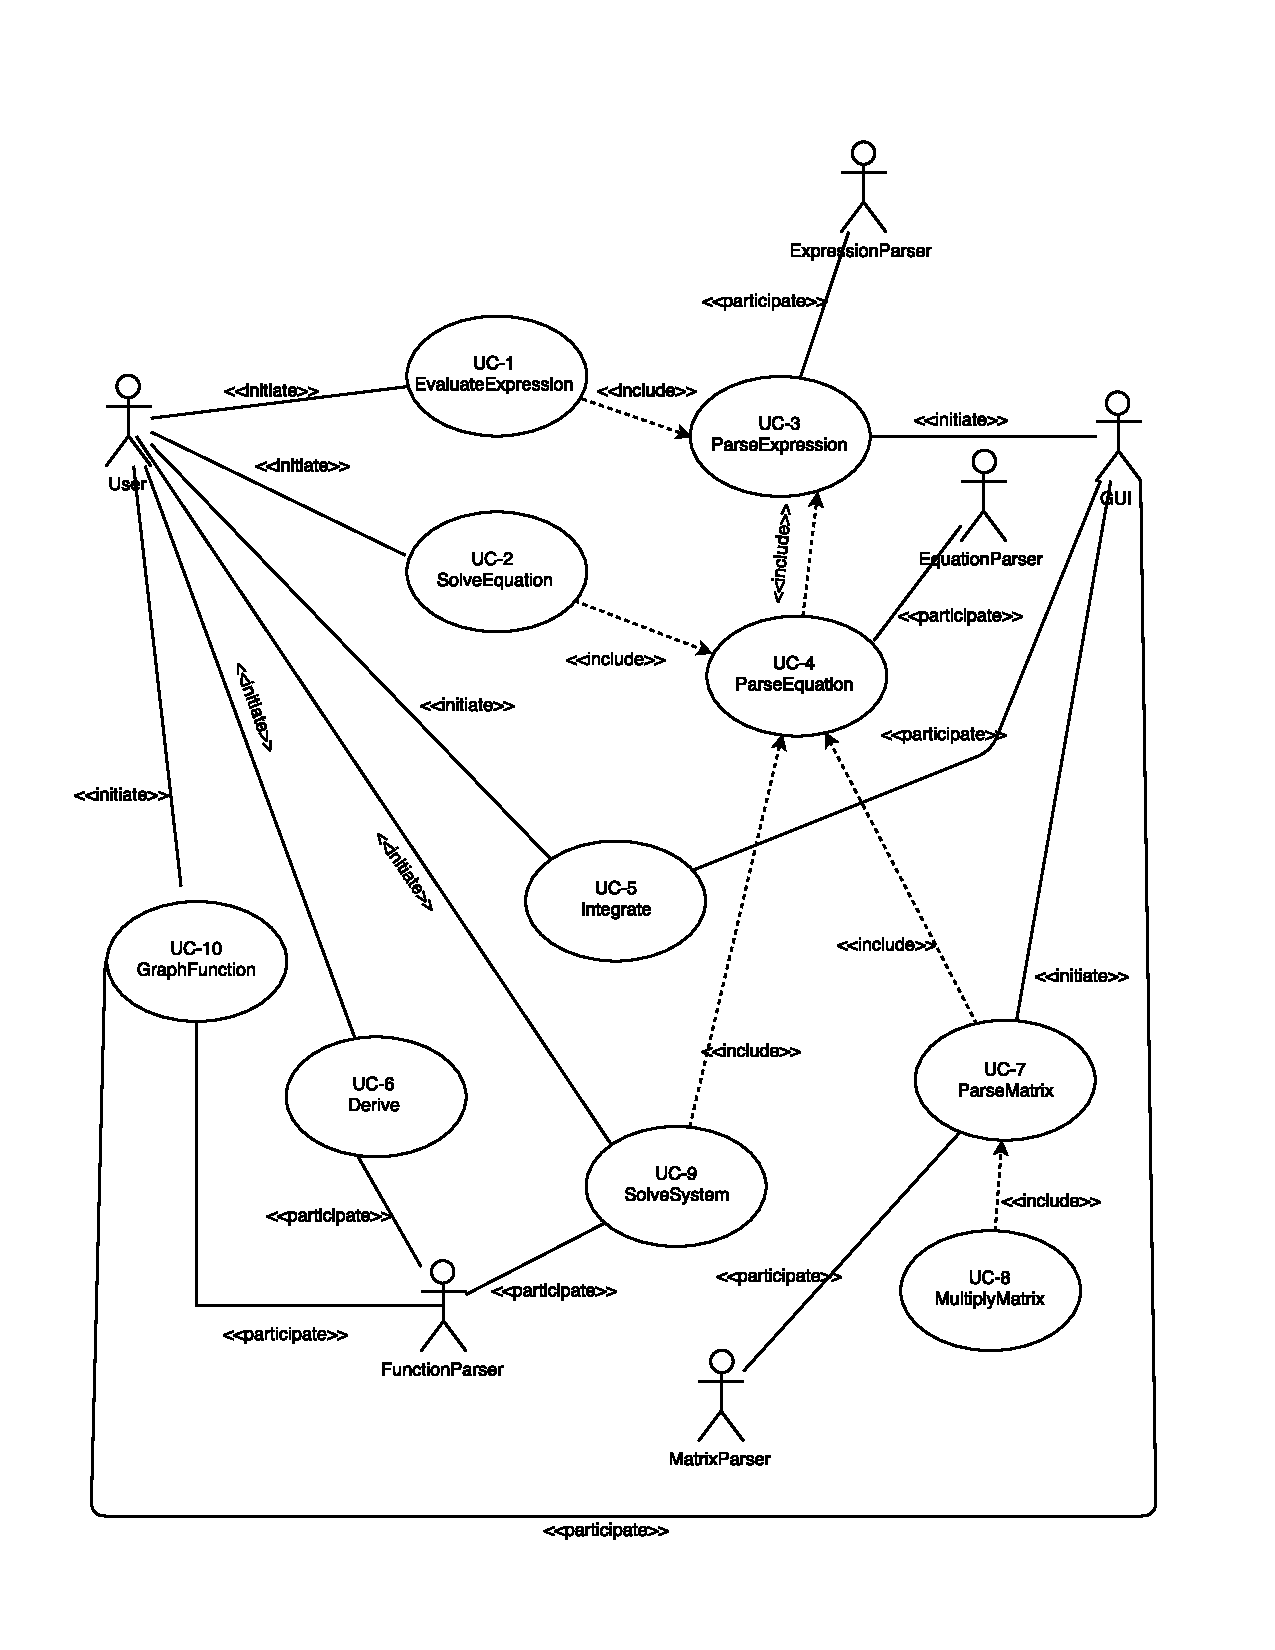
\includepdf[pagecommand={}]{usecasediagram.pdf}

\section{Traceability Matrix}

\begin{center}
\begin{tabular}{|l|l|l|l|l|l|l|l|l|l|l|}
\hline
      & UC-1 & UC-2 & UC-3 & UC-4 & UC-5 & UC-6 & UC-7 & UC-8 & UC-9 & UC-10 \\ \hline
REQ1  & X    &      & X    &      &      &      &      &      &      &       \\ \hline
REQ2  & X    &      &      &      &      &      &      &      &      &       \\ \hline
REQ3  & X    &      &      &      &      &      &      &      &      &       \\ \hline
REQ4  &      & X    &      &      &      &      &      &      &      &       \\ \hline
REQ5  &      & X    &      &  X   &      &      &      &      &      &       \\ \hline
REQ6  &      &      &      &      &  X   & X    &      &      &      &       \\ \hline
REQ7  &      &      &      &      &  X   & X    &      &      &      &       \\ \hline
REQ8  &      &      &      &      &      &      & X    &      &      &       \\ \hline
REQ9  &      &      &      &      &      &      &      & X    &      &       \\ \hline
REQ10 &      &      &      &      &      &      &      &      & X    &       \\ \hline
REQ11 &      &      &      &      &      &      &      &      & X    &       \\ \hline
REQ12 &      &      &      &      &      &      & X    &      &      &       \\ \hline
REQ13 &      &      &      &      &      &      &      &      &      & X     \\ \hline
\end{tabular}
\end{center}

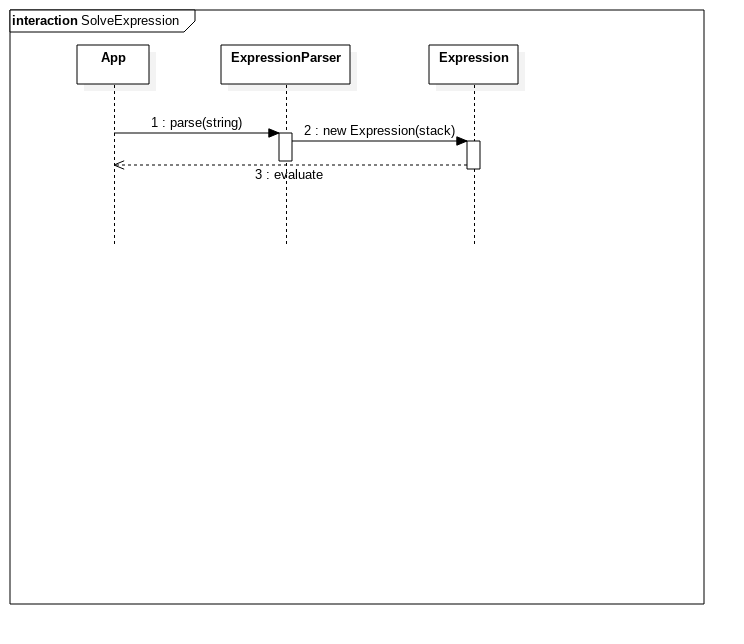
\includepdf[pagecommand={}]{sequencediagrams/sd1.png}
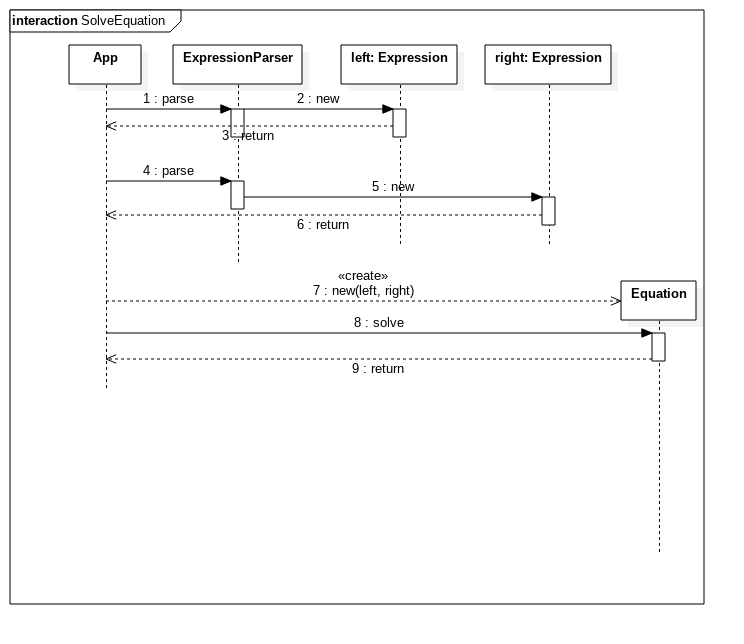
\includepdf[pagecommand={}]{sequencediagrams/sd2.png}
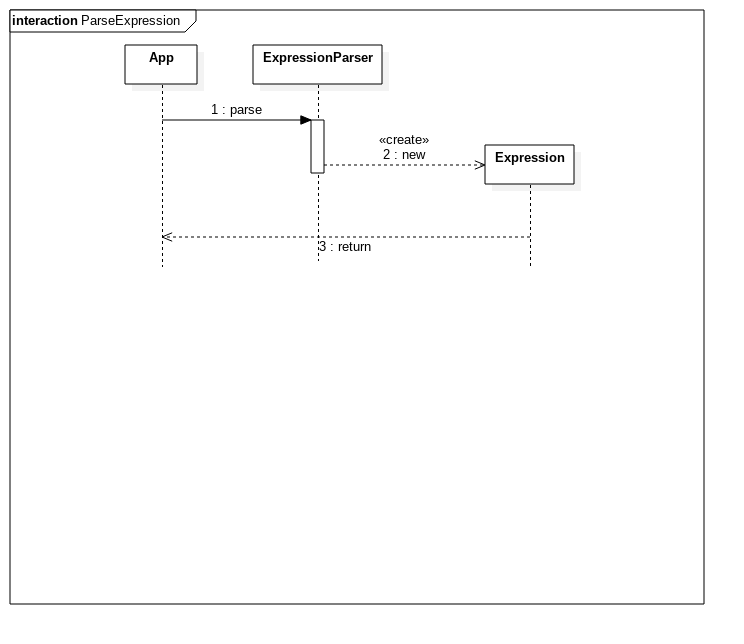
\includepdf[pagecommand={}]{sequencediagrams/sd3.png}
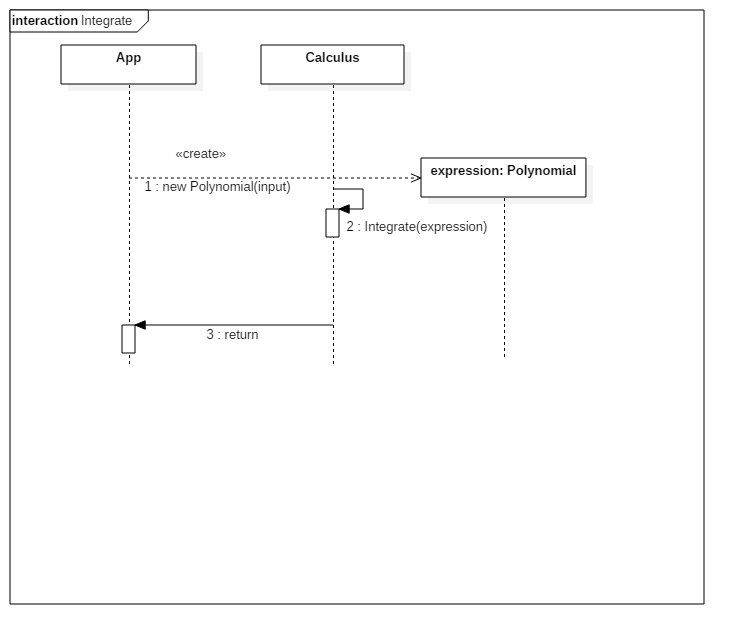
\includepdf[pagecommand={}]{sequencediagrams/sd4.png}
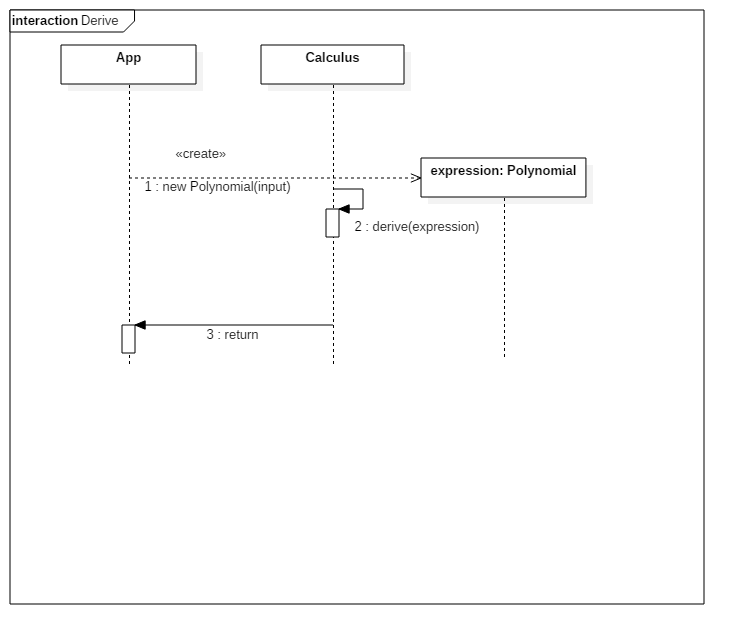
\includepdf[pagecommand={}]{sequencediagrams/sd5.png}
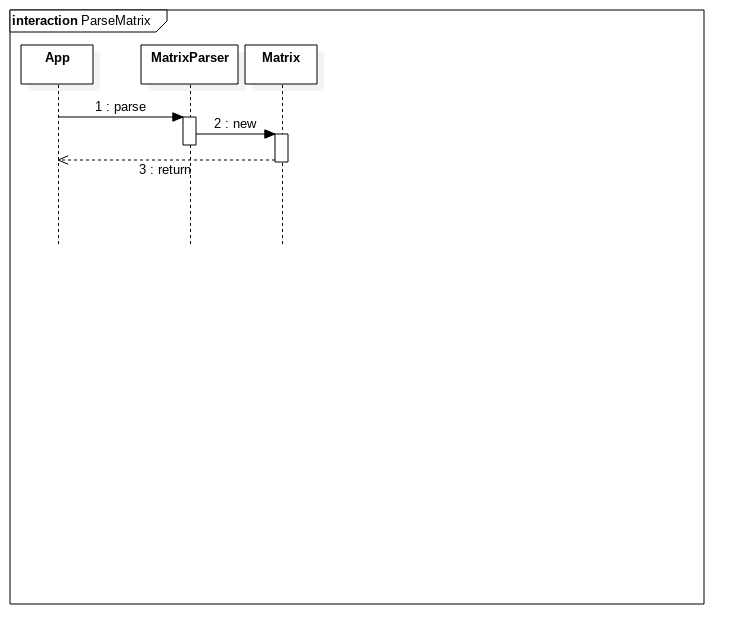
\includepdf[pagecommand={}]{sequencediagrams/sd6.png}
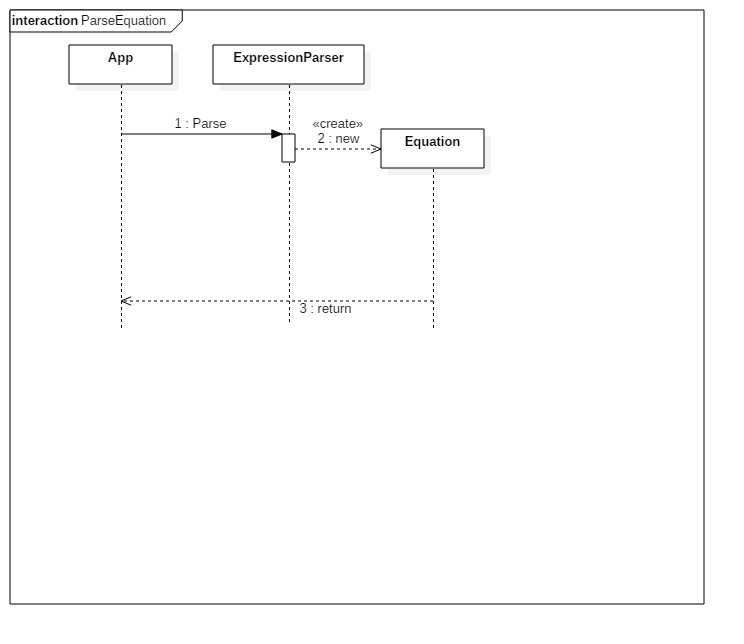
\includepdf[pagecommand={}]{sequencediagrams/sd7.png}
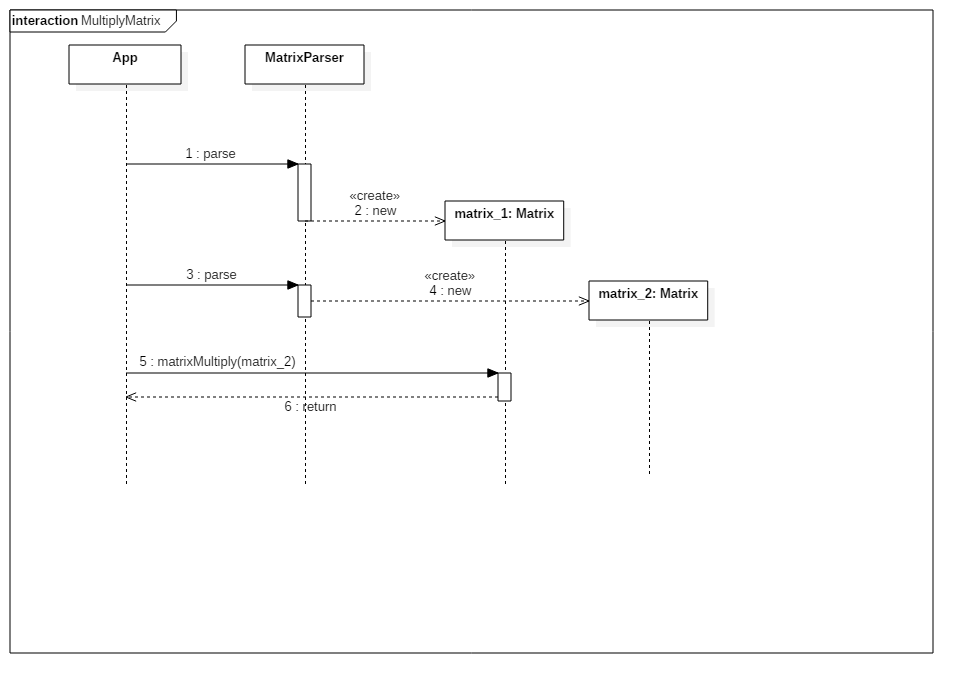
\includepdf[pagecommand={}]{sequencediagrams/sd8.png}
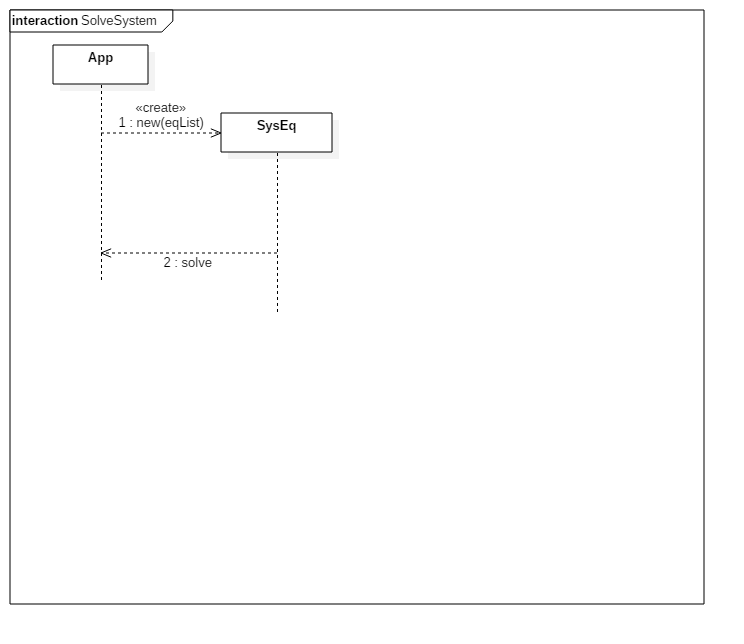
\includepdf[pagecommand={}]{sequencediagrams/sd9.png}

\end{document}
